\documentclass[11pt]{article}
\usepackage[letterpaper,margin=.72in]{geometry}
\usepackage[T1]{fontenc}
\usepackage{lmodern,microtype,graphicx,booktabs,amsmath,hyperref}
\hypersetup{colorlinks=true,urlcolor=blue,pdfauthor={James N. Jean IV},pdftitle={Transit reporting gaps and apparent growth}}
\setlength{\parindent}{0pt}\setlength{\parskip}{6pt}\renewcommand{\arraystretch}{1.1}
\begin{document}
{\Large\bfseries Transit reporting gaps and apparent growth}\par
James N. Jean IV\hfill 29 October 2026\par
\textit{Independent study 07. Not peer reviewed.}
\section*{Decision brief}
When can a year-over-year bus-ridership increase be created by missing reports? This finite comparison tests dashboard summaries against captured published monthly unlinked passenger trips (UPT). Its reporting gaps are synthetic; they are not evidence of actual false agency reports or verified passenger changes.

Fixed stress. Mask prior-year reports from about 10\% of service units chosen by largest 2019 boarding volume. These units account for 74.1--74.5\% of baseline boardings, making this a concentrated-volume stress. Across 36 held months in 2023--2025, zero-fill mean absolute growth error is 319.349 percentage points, count rescaling 276.125 and matched-panel growth 1.289. Zero fill invents positive growth in four months. The matched panel misses one positive-growth month and changes the observed population.

Decision implication. Display reporting coverage, population and volume shares beside growth. Preserve zero, null and absent rows separately. Obtain service-status and reporting-vintage evidence before certifying an increase. Under illustrative twice-2019 component caps, all 972 aggregate intervals contain the benchmark, but 470 cases violate a cap. Containment alone does not validate assumptions.

\begin{center}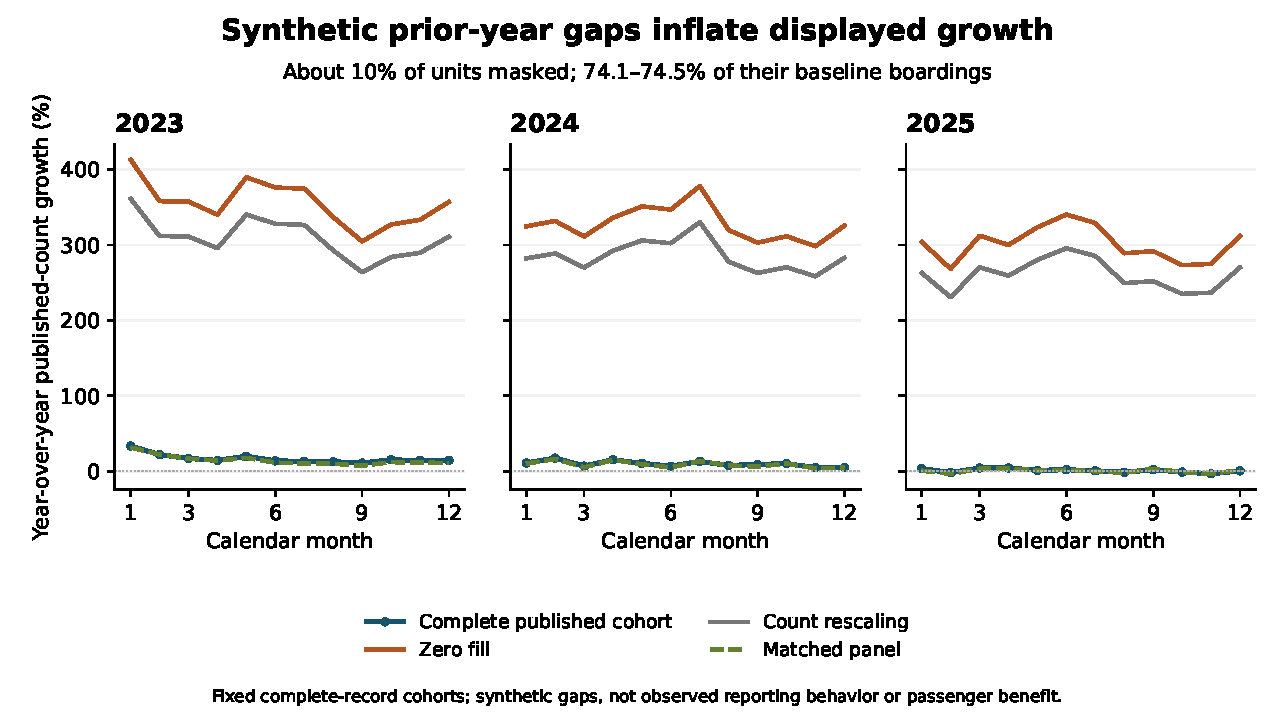
\includegraphics[width=\linewidth]{images/primary_growth.pdf}\end{center}
\small Figure 1. All 36 primary months and four views remain visible. The benchmark is a complete published-record cohort, not passenger truth or prospective evidence. Large errors reflect the concentrated synthetic gap.\normalsize\par

\newpage\section*{1. Source, reporting population and cohort}
The official DOT/FTA Monthly Modal Time Series (5ti2-5uiv) supplies agency, mode, service type and month-level facts [1]. This capture selects MB bus mode and 2019--2025, retrieving only NTD agency ID, service type, year, month timestamp and UPT. Service types remain distinct. The license is public domain; minimal federal facts and original derivatives are attributed. Safety fields, individual passengers, private contacts and full third-party documents are excluded.

The fixed snapshot has 38,584 rows, 50 explicit null UPT entries and 185 reported zeros. Before/after metadata revisions match: row update 1791312691 and view modification 1791312745. Exact requests and response/projection hashes remain available. Independent parsing checks 192,920 projection scalars; separate monthly and agency-year controls reconcile 10,083 count/non-null/sum scalars.

\begin{center}\small\setlength{\tabcolsep}{4pt}
\begin{tabular}{rrrr}\toprule
Year & Published rows & Explicit nulls & Reported zeros \\
\midrule
2019 & 5,544 & 5 & 3 \\
2020 & 5,566 & 4 & 100 \\
2021 & 5,536 & 5 & 32 \\
2022 & 5,473 & 11 & 10 \\
2023 & 5,502 & 14 & 12 \\
2024 & 5,492 & 11 & 12 \\
2025 & 5,471 & 0 & 16 \\
\bottomrule\end{tabular}\end{center}
FTA metadata associates explicit null service entries with late reporting [1]. Absence can reflect entry, exit or scope change and is not asserted to be delinquency. Historical vintages and all estimation/provenance flags are unavailable. This is not claimed to be an original-vintage raw workbook. UPT counts boardings, not unique travelers, latent demand, service reliability or passenger welfare [2,3].

The 2019 roster has 455 agency-service units with twelve known nonnegative integer entries and positive annual UPT. Each target-year benchmark requires all 24 prior/current entries. This complete-case filter excludes incomplete and entering services; it does not establish actual reporting eligibility or national coverage.

\begin{center}\small\setlength{\tabcolsep}{4pt}
\begin{tabular}{rrrrrrr}\toprule
Year & Complete & Excluded & Absent prior & Absent current & Null prior & Null current \\
\midrule
2023 & 416 & 39 & 313 & 396 & 11 & 12 \\
2024 & 410 & 45 & 396 & 501 & 12 & 6 \\
2025 & 403 & 52 & 501 & 566 & 6 & 0 \\
\bottomrule\end{tabular}\end{center}
Absent/null columns count service-month entries within the roster, not agencies or proven late reports. Complete held pairs have 416, 410 and 403 units. Populations differ between years; all inclusion/exclusion records are exported.

\newpage\section*{2. Fixed comparisons and primary results}
Protocol c6757eb predates count retrieval. Development targets are 2020--2022; held targets are 2023--2025. Eighteen source/protocol/executable dependencies from 5df3333 are publicly frozen in 6d32b93 before held analytical summaries. Raw source values and quality are visible without blinding. Complete-pair eligibility uses later captured records, so this is retrospective rather than a prospective availability test. No model, tuning winner or policy is selected.

Mask ceil(pN) units for p = 1/20, 1/10 or 1/5. Rank by 2019 annual volume descending, ascending or identifier; ties use agency ID then service type. Remove all twelve months in the prior year, current year or both. These 27 deterministic persistent blocks are synthetic stress cases, not random samples or estimated missingness mechanisms. The primary setting is 10\%, largest-baseline units and prior-year-only gaps.

For complete prior/current totals B,A, growth is A/B\ensuremath{-}1 when B>0. Zero fill uses observed sums. Count rescaling multiplies each period sum by full/observed unit count. Matched-panel growth uses the same observed units in both periods. Zero reference denominators yield explicitly undefined percentages. The matched view changes population; count rescaling assumes representative missing units. Neither is guaranteed unbiased.

Errors are percentage points against the complete published cohort. Each year weights 12 months equally; pooled weights all 36. False growth means estimate>0 with benchmark\ensuremath{\leq}0; missed growth means estimate\ensuremath{\leq}0 with benchmark>0. Zero has a distinct sign.

\begin{center}\small\setlength{\tabcolsep}{4pt}
\begin{tabular}{llrrrr}\toprule
Year & View & MAE (pp) & Sign errors & False growth & Missed growth \\
\midrule
2023 & Zero fill & 338.996 & 0 & 0 & 0 \\
2023 & Count rescaled & 292.988 & 0 & 0 & 0 \\
2023 & Matched panel & 2.132 & 0 & 0 & 0 \\
2024 & Zero fill & 318.408 & 0 & 0 & 0 \\
2024 & Count rescaled & 275.594 & 0 & 0 & 0 \\
2024 & Matched panel & 0.938 & 0 & 0 & 0 \\
2025 & Zero fill & 300.642 & 4 & 4 & 0 \\
2025 & Count rescaled & 259.792 & 4 & 4 & 0 \\
2025 & Matched panel & 0.795 & 1 & 0 & 1 \\
Pooled & Zero fill & 319.349 & 4 & 4 & 0 \\
Pooled & Count rescaled & 276.125 & 4 & 4 & 0 \\
Pooled & Matched panel & 1.289 & 1 & 0 & 1 \\
\bottomrule\end{tabular}\end{center}
Primary masks contain 42/416, 41/410 and 41/403 units, representing 74.515\%, 74.113\% and 74.444\% of baseline volume. Across all 972 held settings, the matched view has lower absolute error than zero fill in 648 and equal error in 324. Both-period masks give identical point views because they retain the same units. No universal estimator superiority follows.

\newpage\section*{3. Every declared gap setting}
Every cell is mean absolute growth error in percentage points across 36 held months. Fractions count units, not volume. No ranking, fraction or missing-year side is discarded because of its result. Exact monthly growth, signed/squared errors, masks and denominators remain in the exports.

\begin{center}\small\setlength{\tabcolsep}{4pt}
\begin{tabular}{rllrrr}\toprule
Units (\%) & Rank rule & Missing year(s) & Zero fill & Rescaled & Matched \\
\midrule
5 & Largest baseline & Prior & 180.929 & 166.068 & 1.477 \\
5 & Largest baseline & Current & 68.526 & 66.335 & 1.477 \\
5 & Largest baseline & Both & 1.477 & 1.477 & 1.477 \\
5 & Smallest baseline & Prior & 0.030 & 5.561 & 0.004 \\
5 & Smallest baseline & Current & 0.031 & 5.859 & 0.004 \\
5 & Smallest baseline & Both & 0.004 & 0.004 & 0.004 \\
5 & Identifier & Prior & 5.304 & 0.557 & 0.191 \\
5 & Identifier & Current & 5.238 & 0.382 & 0.191 \\
5 & Identifier & Both & 0.191 & 0.191 & 0.191 \\
10 & Largest baseline & Prior & 319.349 & 276.125 & 1.289 \\
10 & Largest baseline & Current & 81.547 & 78.455 & 1.289 \\
10 & Largest baseline & Both & 1.289 & 1.289 & 1.289 \\
10 & Smallest baseline & Prior & 0.120 & 10.898 & 0.007 \\
10 & Smallest baseline & Current & 0.123 & 12.105 & 0.007 \\
10 & Smallest baseline & Both & 0.007 & 0.007 & 0.007 \\
10 & Identifier & Prior & 10.514 & 1.553 & 0.251 \\
10 & Identifier & Current & 9.660 & 1.497 & 0.251 \\
10 & Identifier & Both & 0.251 & 0.251 & 0.251 \\
20 & Largest baseline & Prior & 665.585 & 509.878 & 1.511 \\
20 & Largest baseline & Current & 93.766 & 89.907 & 1.511 \\
20 & Largest baseline & Both & 1.511 & 1.511 & 1.511 \\
20 & Smallest baseline & Prior & 0.515 & 21.518 & 0.012 \\
20 & Smallest baseline & Current & 0.515 & 26.801 & 0.012 \\
20 & Smallest baseline & Both & 0.012 & 0.012 & 0.012 \\
20 & Identifier & Prior & 66.045 & 30.842 & 1.202 \\
20 & Identifier & Current & 41.731 & 24.783 & 1.202 \\
20 & Identifier & Both & 1.202 & 1.202 & 1.202 \\
\bottomrule\end{tabular}\end{center}
A count adjustment cannot recover an informatively missing volume share by assumption alone. Both-period masks produce identical point views because the same unit set and count scaling apply to numerator and denominator. Their common error may remain nonzero because the observed panel differs from the full benchmark.

\newpage\section*{4. Composition and cap assumptions}
\begin{center}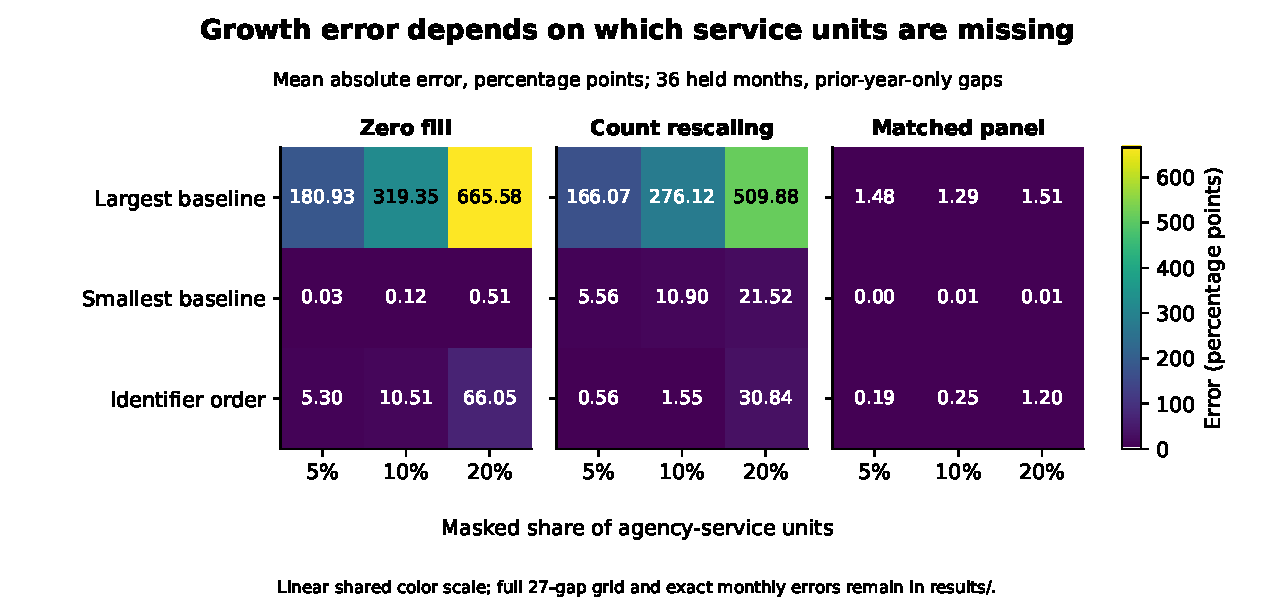
\includegraphics[width=\linewidth]{images/gap_sensitivity.pdf}\end{center}
\small Figure 2. All nine prior-year-only settings use a shared linear scale. Other year-side settings remain in the complete table. Text shows values visually compressed by that scale; rounding a small error to 0.00 does not make it exactly zero.\normalsize\par

For each hidden component, assume a nonnegative count capped at gamma times its same-calendar-month 2019 UPT. Use gamma equal to 1, 2 or 4. These untuned sensitivity caps are not measured capacities or confidence bounds. A positive hidden value violates any multiplier of a zero baseline. Nonnegativity alone supplies no finite missing-count upper bound.

Each group below has 324 cases: three fractions, three rankings and 36 months. Inside means complete-cohort growth lies in the aggregate interval. Valid means every hidden component satisfies its cap. Component violations repeat across scenarios and are not unique service-months.

\begin{center}\small\setlength{\tabcolsep}{4pt}
\begin{tabular}{rlrrrr}\toprule
Multiplier & Missing year(s) & Cases & Inside & Valid & Violating components \\
\midrule
1 & Prior & 324 & 314 & 31 & 2347 \\
1 & Current & 324 & 309 & 0 & 3214 \\
1 & Both & 324 & 324 & 0 & 5561 \\
2 & Prior & 324 & 324 & 192 & 204 \\
2 & Current & 324 & 324 & 157 & 312 \\
2 & Both & 324 & 324 & 153 & 516 \\
4 & Prior & 324 & 324 & 214 & 134 \\
4 & Current & 324 & 324 & 168 & 189 \\
4 & Both & 324 & 324 & 164 & 323 \\
\bottomrule\end{tabular}\end{center}
At multiplier 2, all 972 aggregate intervals contain the benchmark but only 502 cases satisfy every component cap; 470 fail an assumption. At multiplier 4, only 546 cases satisfy all caps. High finite containment and looser caps do not establish future coverage.

\newpage\section*{5. Conditional bounds and important limits}
\begin{center}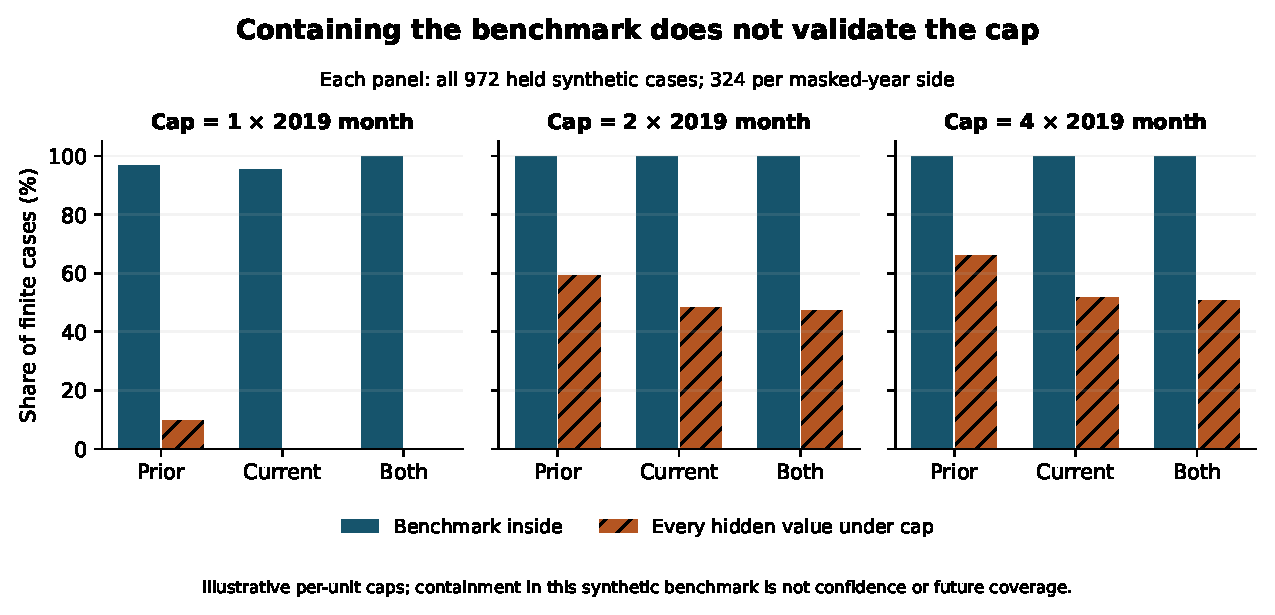
\includegraphics[width=\linewidth]{images/bound_assumptions.pdf}\end{center}
\small Figure 3. Aggregate containment and component-cap validity are distinct checks. Every panel includes all 972 held cases, with 324 per year-side group. These constructed finite rates are not probabilistic coverage estimates.\normalsize\par

Sum known values and component ranges into prior B in [BL,BU] and current A in [AL,AU]. For positive reference endpoints, monotonicity gives growth in [AL/BU\ensuremath{-}1,AU/BL\ensuremath{-}1]. If BL=0<BU and AU>0, the upper endpoint is unbounded. If BU=0, reference growth is undefined. A zero current upper bound gives \ensuremath{-}1 for any admissible positive reference. All endpoint states are explicit. Observed cap violations block assumption-supported positive-growth certificates.

Real missing values are unknown, so their cap validity generally cannot be checked. This experiment conditions on complete published records and deliberately informative persistent gaps. It does not estimate how often agencies report late, how closures affect coverage or how another missingness mechanism behaves.

UPT can be revised, estimated or measured imperfectly. Controls check publication consistency, not passenger truth. Scope omits some providers and cannot represent all transit. No historical-vintage availability, random-sampling, causal, passenger-benefit, deployment, realized-savings, peer-review or exhaustive novelty claim follows. Finite errors and containment rates are not confidence intervals or guarantees for future missing data.

\newpage\section*{6. Reproduction and evidence status}
Sixteen fixtures cover zero/null/absence, duplicate keys, service separation, mask rounding, ranking ties, both-period gaps, signs and finite/unbounded/undefined endpoints. Independent checkers import no production model or summary helpers. SQL constraints, grouped eligibility and window rankings reconstruct cohorts/masks; separate integer/rational arithmetic checks every point and bound row.

Development and held exports pass 172,866 and 171,408 exact scalar checks; all summary fields add 2,160. Isolated replay matches 346,434 CSV fields and three verification documents and checks 18 protected dependencies. Original runtimes remain exported; variable replay times are excluded from deterministic identity. No regression estimator, optimizer, stochastic seed or fine-tuning run is used. Fractions, ranks, sides and caps are fixed protocol choices, not empirically tuned settings.

The original figures have 333 actual artist-value checks, 27 annotation/contrast checks and nine hashes. Rendered readability checks do not establish accessibility conformance. Reproduce from the repository root:

\begin{quote}\small\begin{verbatim}
python -m pip install -r requirements.txt
python -m unittest discover -s tests -v
python src/check_reproduction.py
python src/verify_summaries.py
python src/verify_figures.py
python src/verify_paper.py
python src/verify_public_package.py
\end{verbatim}\end{quote}
Replay uses captured facts rather than silently requesting later data. Release additionally requires scoped canonical/privacy checks, exact-head Linux success and matching merged tree/annotated tag. Independent program work, not peer reviewed. Formal-publication projects, including Azure optimization, remain private.

\section*{References}\small
[1] U.S. DOT/FTA. \href{https://data.transportation.gov/Public-Transit/Monthly-Modal-Time-Series/5ti2-5uiv}{Monthly Modal Time Series}; public-domain metadata, service fields and null-reporting description. Accessed 29 October 2026; exact requests/hashes/revisions in the manifest.\par
[2] FTA. \href{https://www.transit.dot.gov/ntd/monthly-ridership}{Monthly Ridership}; population, measures and separate raw/adjusted products. The portal snapshot is identified separately.\par
[3] BTS. \href{https://www.bts.gov/learn-about-bts-and-our-work/statistical-methods-and-policies/public-transit-ridership}{Public Transit Ridership Used in the Transportation Services Index}; revision, coverage and counting limitations. Accessed 29 October 2026.
\end{document}
